\documentclass{beamer}

\usetheme{metropolis}

\usepackage{xparse}
\usepackage{xfrac}
\usepackage[siunitx, american]{circuitikz}
\usepackage{hyperref}
\usepackage{cancel}
\usepackage{amssymb}
\usepackage{amsmath}
\usepackage{graphicx}
\usepackage{spalign}
\usetikzlibrary{automata, arrows}

% https://tex.stackexchange.com/questions/2233/whats-the-best-way-make-an-augmented-coefficient-matrix
\makeatletter
\renewcommand*\env@matrix[1][*\c@MaxMatrixCols c]{%
  \hskip -\arraycolsep
  \let\@ifnextchar\new@ifnextchar
  \array{#1}}
\makeatother


% https://tex.stackexchange.com/questions/102069/make-a-heading-in-beamer
\newcommand\makeheader[1]{%
  \par\bigskip
  {\large\bfseries#1}\par\smallskip}

\title{EECS 16A Midterm 1 Review Session}
\author{Presented by \textless NAMES \textgreater (HKN)}
\date{}




\begin{document}

\begin{frame}

\titlepage

\end{frame}

\begin{frame}[t]\vspace{20pt}
\frametitle{Disclaimer}
Although some of the presenters may be course staff, the material covered in the review session may not be an accurate representation of the topics covered in and difficulty of the exam.

\vspace{20pt}
Slides are posted at --- on Piazza.

\end{frame}


\begin{frame}[t]\vspace{20pt}
\frametitle{HKN Drop-In Tutoring}

\begin{itemize}
\item These details should be edited
\end{itemize}

\end{frame}

\section*{Systems of Equations and Gaussian Elimination}

\begin{frame}[t]\vspace{20pt}
\frametitle{Vectors}
Conceptually, a vector is a collection of numbers that each represent a variable. If there are $n$ variables, then the vector is $n$-dimensional.

Example: \newline
A point in 3D can be represented as $(x,y,z)$
In vector form, this would be represented as $\begin{bmatrix} x \\ y \\ z \\ \end{bmatrix}$

\end{frame}


\begin{frame}[t]\vspace{5pt}
\frametitle{Matrices}
\begin{itemize}
\item Collection of \textbf{vectors}
\item 2D table for \textbf{storing data}
	\begin{itemize}
		\item[$\circledcirc$] Systems of equations for imaging observations
	\end{itemize}
\item Notable/useful matrices
	\begin{itemize}
		\item[$\circledcirc$] Identity matrix
		\item[$\circledcirc$] Augmented matrices
		\item[$\circledcirc$] Rotation matrix
		\item[$\circledcirc$] Many others!
	\end{itemize}
\end{itemize}

Augmented:
$\begin{bmatrix}[ccc|c]
1 & -2 & 3 & 7\\
2 & 1 & 1 & 4\\
-3 & 2 & 3-2& 10\\
\end{bmatrix}$

Rotation: \hspace{9pt}
$\begin{bmatrix}
\cos{\theta} & -\sin{\theta} \\
\sin{\theta} & \cos{\theta} \\

\end{bmatrix}$

\end{frame}



\begin{frame}[t]\vspace{10pt}
\frametitle{Matrix Transformations}

Matrices are often used to perform transformations, especially 
\newline in $\mathbb{R}^2$ \\~\\
Two important transformations:

\begin{figure}[!tbp]
  \centering
  \begin{minipage}[b]{0.3\textwidth}
    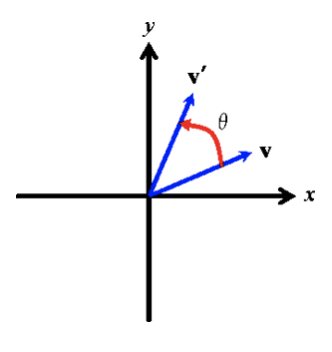
\includegraphics[width=\textwidth]{./images/rotation.png}
    \caption{Rotation}
  \end{minipage}
  \hfill
  \begin{minipage}[b]{0.3\textwidth}
    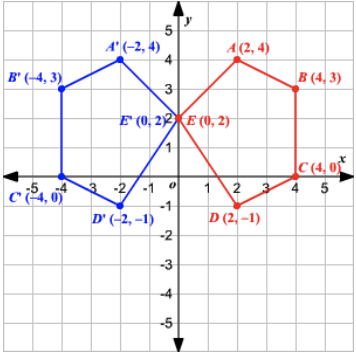
\includegraphics[width=\textwidth]{./images/reflection.png}
    \caption{Reflection}
  \end{minipage}
\end{figure}
\end{frame}



\begin{frame}[t]\vspace{10pt}
\frametitle{Rotation Matrix}
The rotation matrix rotates points by a specified angle, theta: \\~\\
$R(\theta) = \begin{bmatrix}
\cos{\theta} & -\sin{\theta} \\
\sin{\theta} & \cos{\theta} \\
\end{bmatrix}$

Use this matrix by plugging in desired rotation angle, then multiply with vector. \\
\textbf{Note: } Rotation matrices also preserve the length of a vector. \\~\\
\textbf{Example}: Rotation Matrix that rotates vector by $90^{\circ}$ \\~\\
$R(90^{\circ}) = \begin{bmatrix}
0 & -1 \\
1 & 0 \\
\end{bmatrix}$
\end{frame}

\begin{frame}[t]\vspace{10pt}
\frametitle{Rotation Matrix}
The rotation matrix rotates points by a specified angle, theta: \\~\\
$R(\theta) = \begin{bmatrix}
\cos{\theta} & -\sin{\theta} \\
\sin{\theta} & \cos{\theta} \\
\end{bmatrix}$

Use this matrix by plugging in desired rotation angle, then multiply with vector. \\
\textbf{Note: } Rotation matrices also preserve the length of a vector. \\~\\
\textbf{Example}: Rotation Matrix that rotates vector by $90^{\circ}$ \\~\\
$R(90^{\circ}) = \begin{bmatrix}
0 & -1 \\
1 & 0 \\
\end{bmatrix}$
\end{frame}

\begin{frame}[t]\vspace{10pt}
\frametitle{Reflection Matrix}

The reflection matrix reflects vectors across a line (Notice that such matrix also preserves the length of a vector)\\~\\
Notable reflection matrices:

\begin{figure}
  \begin{minipage}{.5\linewidth}
    \centering
    \[\left[\begin{array}{cc}
      1 &  0\\
      0 & -1
    \end{array}\right]\]
    Reflection across $x$-axis
  \end{minipage}%
  \begin{minipage}{.5\linewidth}
    \centering
    \[\left[\begin{array}{cc}
      -1 &  0\\
      0 & 1
    \end{array}\right]\]
    Reflection across $y$-axis
  \end{minipage}
  \begin{minipage}{.5\linewidth}
    \centering
    \[\left[\begin{array}{cc}
      0 & 1\\
      1 & 0
    \end{array}\right]\]
    Reflection across $y=x$
  \end{minipage}
\end{figure}
\end{frame}



\begin{frame}[t]\vspace{10pt}
\frametitle{Matrix Transformations}
All linear transformations can be expressed as a matrix

\begin{figure}[!tbp]
  \centering
  \begin{minipage}[b]{0.45\textwidth}
    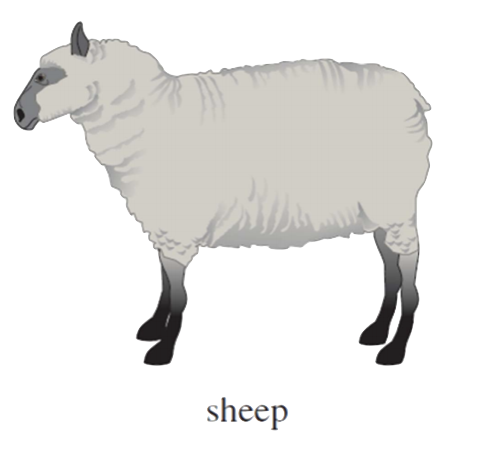
\includegraphics[width=\textwidth]{./images/sheep.png}
  \end{minipage}
  \hfill
  \begin{minipage}[b]{0.45\textwidth}
    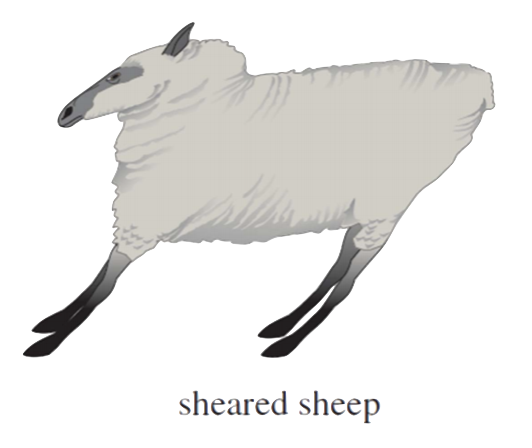
\includegraphics[width=\textwidth]{./images/sheep_shear.png}
  \end{minipage}
\end{figure}
\end{frame}


\begin{frame}[t]\vspace{-10pt}
\frametitle{Example 1}
\only<1>{\makeheader{Question}}
\only<2>{\makeheader{\textcolor{red}{Solution}}}

What is the resulting vector after the following (non-subsequent) transformations are applied 
to the vector 
$\vec{v}= \begin{bmatrix}
2 \\ 3
\end{bmatrix}$
\\~\\

\begin{enumerate}
\setcounter{enumi}{0}
\item Rotate by $45^{\circ}$
\end{enumerate}

\only<1>{\vspace{30pt}}

\only<2>{
\vspace{-10pt}
\[
\begin{bmatrix}
    \cos{45^{\circ}}  &  -\sin{45^{\circ}}      \\
    \sin{45^{\circ}}  &  \cos{45^{\circ}}    
\end{bmatrix}
= 
\begin{bmatrix}
    \frac{\sqrt{2}}{2}  &  -\frac{\sqrt{2}}{2}      \\
    \frac{\sqrt{2}}{2}  &  \frac{\sqrt{2}}{2}      
\end{bmatrix} 
\begin{bmatrix}
    2 \\ 3
\end{bmatrix} 
=
\begin{bmatrix}
 - \frac{\sqrt{2}}{2} \\
 	\frac{5\sqrt{2}}{2}
\end{bmatrix}
\]

}

\begin{enumerate}
\setcounter{enumi}{1}
\item Reflect across $y = x$
\end{enumerate}

\only<2>{
\vspace{-10pt}
\[
\begin{bmatrix}
    0 & 1 \\ 1 & 0
\end{bmatrix} 
\begin{bmatrix}
    2 \\ 3
\end{bmatrix} 
=
\begin{bmatrix}
 3\\2
\end{bmatrix}
\]
}
\end{frame}


\begin{frame}[t]\vspace{10pt}
\frametitle{Determinants}
Determinant of a $2 x 2$ matrix: \\
\[ 
det \, (
\begin{bmatrix} a & b \\ c & d \end{bmatrix}
)
= ad - bc
\]

Also, an upper triangular matrix’s determinant is the product of the diagonal: \\
\[ 
det \, (
\begin{bmatrix} 
a & * & * & \cdots \\
0 & b & * & \cdots \\
0 & 0 & c & \cdots \\
\vdots & \vdots & \vdots & \ddots \\
 \end{bmatrix}
)
= abc \cdots
\]
\end{frame}



\begin{frame}[t]\vspace{10pt}
\frametitle{Gaussian Elimination}
\textbf{Ultimate goal: } Upper triangular form (\textbf{i.e} numbers below the diagonal are all 0) \\~\\
\textbf{Reminder of Motivation:} Can work starting from the bottom row up in order to quickly calculate (from a computer’s perspective) each variable’s value. \\
For example, the last row has one variable and one value. 
\end{frame}


\begin{frame}[t]\vspace{10pt}
\frametitle{Gaussian Elimination}
\textbf{IDEA: } Augmented matrix represents a system of equations where each row is an equation. \\
What are you allowed to do with equations to solve them?

\begin{enumerate}
\item \textbf{Row exchange} (same equations,  different order)
\item \textbf{Scaling} (multiplying an equation by  a scalar)
\item \textbf{Replace a row with the a linear combination of itself and another row} (intuitively, must include itself because otherwise there is “loss of information”, like a deletion of one of the original rows)
\end{enumerate}

\textbf{GOAL:} \\ Original Matrix $\rightarrow$ Row Echelon Form $\rightarrow $ Reduced Row Echelon Form
\end{frame}


\begin{frame}[t]\vspace{-10pt}
\frametitle{Gaussian Elimination Example}
\only<1>{\makeheader{Problem}}
\only<2>{\makeheader{\textcolor{red}{Solution}}}
Use Gaussian Elimination to reduce the following system of equations:\\~\\

% https://tex.stackexchange.com/questions/35174/best-way-to-create-an-system-of-equations-environment
\only<1> {
\[
  \spalignsys{
    x_1 +  x_2 + x_3 = 8;
    2x_1 - 4x_2 +  3x_3 =  9 ;
    -x_1 + 5x_2 - 2x_3 = 0
  }
\]
}
\only<2>{
$
  \begin{bmatrix}[ccc|c]
  1 & 1 & 1 & 8\\
  2 & -4 & 3 & 9\\
  -1 & 5 & -2 & 0
  \end{bmatrix}
  \xrightarrow[]{2R_1 - R_2 \rightarrow R_2 }
  \begin{bmatrix}[ccc|c]
  1 & 1 & 1 & 8\\
  0 & 6 & -1 & 7\\
  -1 & 5 & -2 & 0
  \end{bmatrix}
  \xrightarrow[]{R_1 + R_3 \rightarrow R_3 }
$

\vspace{10pt}

$
  \begin{bmatrix}[ccc|c]
   1 & 1 & 1 & 8\\
   0 & 6 & -1 & 7\\
   0 & 6 & -1 & 8
  \end{bmatrix}
  \xrightarrow[]{R_2 - R_3 \rightarrow R_3  }
  \begin{bmatrix}[ccc|c]
  1 & 1 & 1 & 8\\
   0 & 6 & -1 & 7\\
  0 & 0 & 0 & -1
  \end{bmatrix} 
$

The last row implies 0 of three variables add up to -1. Therefore, there exists no solution.
}
\end{frame}


\begin{frame}[t]\vspace{10pt}
\frametitle{Possible Outcomes from Gaussian Elimination}

\hspace*{-2pt}\makebox[\linewidth][c]{
\begin{tiny}
\begin{tabular}{p{2.5cm} | p{2.5cm} | p{2.5cm} | p{2.5cm}}

\textbf{Possible Results} & Row Picture & Column Picture & Properties of Matrix A\\
\hline \hline
\textbf{Unique solution} & Equations intersect at exactly one point & \textbf{b} can be uniquely represented by the linear combination of the columns of  \textbf{A} &  \textbf{A} is invertible \\
\hline
\textbf{Infinite solutions} & Equations intersect along an infinite space (eg. the intersection is a line or a plane) & There are multiple ways of representing \textbf{b} in terms of the linear combination of the columns of \textbf{A} & \textbf{A} has linearly dependent columns \\
\hline
\textbf{No solutions} & Equations do not intersect & \textbf{b} is not in the span of the columns of \textbf{A}; \textbf{b} is not in the column space of \textbf{A} & Column space of \textbf{A} does not contain (span) the vector \textbf{b}
\end{tabular}
\end{tiny}
}


\end{frame}


\end{document}